\section{Lokal optimal løsning}
Når først en optimal løsning er fundet, er det nødvendigt at tjekke, at der ikke er tale om en lokal optimal løsning.
\begin{defn}[Lokalt optimal løsning]
Lad $\vec{x} \in P$ være en løsnings til et lineært programerigns problem med objektfunktion $f$ da er $\vec{x}$ en lokal optimal løsning, hvis $f(\vec{x}) \leq f(\vec{y})$ for $|\vec{y}-\vec{x}|< \epsilon$ for et $\epsilon > 0$ og $\vec{y} \in P$.
\end{defn}
Betragt beviset for Sætning \ref{stn:eksistens}, her konstrueres hele tiden en mere optimal løsning end den foregående, ved at lægge et multiplum af en retningsvektor til den originale vektor, så en ny betingelse blev aktiv.
Der vil derfor kunne opstå et lokalt minimum, hvis der ikke eksistere en sådan retningsvektor, men der er en løsning som er mere optimal, se Figur \ref{fig:lokaltmin}.
\begin{figure}
\begin{center}
	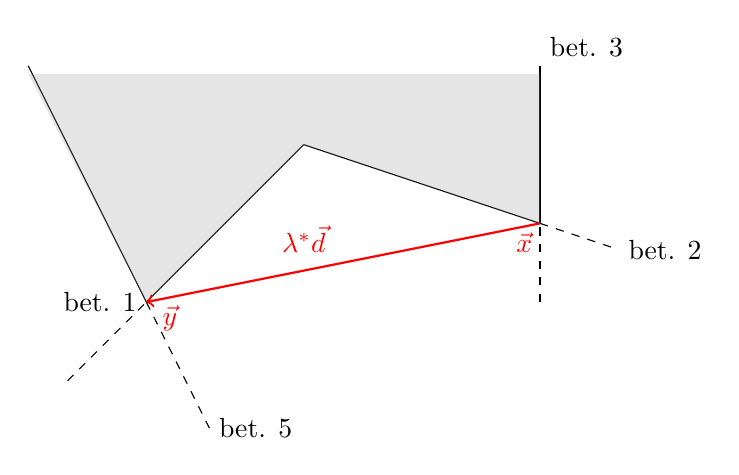
\begin{tikzpicture}[ latex
  s/.style={width=0}]

  %ligning 1
	\draw[domain=-1:0,variable=\x,dashed] 	plot({\x},{\x})  node[left] {bet. 1};
	\draw[domain=0:2,variable=\x] 			plot({\x},{\x});

	
  %ligning 2
	\draw[domain=2:5,variable=\x] 			plot({\x},{-(1/3)*\x+8/3});
	\draw[domain=5:6,variable=\x,dashed] 	plot({\x},{-(1/3)*\x+8/3}) node[right] {bet. 2};
	

  %ligning 3
	\draw[domain=0:1,variable=\y, dashed] 			plot({5},{\y});
	\draw[domain=1:3,variable=\y] 	plot({5},{\y}) node[above right] {bet. 3};
	

	
  %ligning 5
  	\draw[domain=-1.5:0,variable=\x] 	plot({\x},{-2*\x}) ;
	\draw[domain=-0:4/5,variable=\x, dashed] 			plot({\x},{-2*\x}) node[right] {bet. 5} ;


  %løsningsmængden skraveret
	\fill[gray!80,nearly transparent]  (0,0) -- (2,2) -- (5,1) -- (5,2.9) --(-1.5,2.9) --  cycle;
	
  % vektor x
  \node[thick, color=red] (x) at (4.8,0.75) {$\vec{x}$};
  
\node[thick, color=red] (y) at (0.3,-0.2) {$\vec{y}$};
%   %\node[s] (d) at (2, -0.5);
 \draw[thick, color=red, ->](5,1) -- (0,0) node[above, yshift=0.5 cm, xshift=2 cm] {$\lambda^* \vec{d}$} ;
%   \node[] (x) at (2.1, -0.6) {$\vec{x}+\lambda^* \vec{d}$};
%  % \path (x) edge node[right] {$\vec{x}+\lambda^* \vec{d}$} (d) ;
 
\end{tikzpicture}
	\captionof{figure}{Bemærk at der ikke eksistere en retningsvektor $\vec{d}$, så der kan konstueres en bedre løsning, uden at overskride betingelse $2$, derfor vil løsningsvektor $\vec{x}$ fremstå optimal, selvom at løsningsvektor $\vec{y}$ er mere optimal. Løsningsvektor $\vec{x}$ er et lokalt minimum.}
	\label{fig:lokaltmin}
\end{center}
\end{figure}
Det er dog ikke alle mængder, hvor der kan forekomme lokale optimale løsninger, ved fremgangsmåden fra beviset for Sætning \ref{stn:eksistens}.
\begin{defn} [Konveks mængde]
Lad $S \subset \mathds{R}^n$  da er $S$ konveks, hvis der $\forall \vec{x}, \vec{y} \in S$ og et vilkårligt $\lambda \in [0,1]$ gælder at $\lambda \vec{x} + (1-\lambda) \vec{y} \in S$.
\label{def:Konveks}
\end{defn}
En konveksmængde er en mængde der opfylder at det vægtede gennemsnit af et hvert par af elementer også tilhører mængden, det betyder at der altid kan findes en retningsvektor mellem et hvert punkt i mængden.
Helt generelt gælder det, hvis løsningsmængden til et lineært ligningsproblem er konveks, så vil en hver lokal optimal løsning, være en optimal løsning.
\begin{stn}
Lad $\vec{x} \in P$ være en lokal optimal løsnings til et lineært programerignsproblem  med objektfunktion $f$.
Da er  $f(\vec{x}) \leq f(\vec{y})$ for alle $\vec{y} \in P$ hvis $P$ er konveks.
\end{stn}
\begin{proof}
Antag at $\vec{x}^* \in P$ er en optimal løsning.
Da $P$ er konveks medfører det at $\lambda \vec{x}^* + (1-\lambda)\vec{x} \in P$. 
Da $\lambda$ kan vælges til at være vilkårligt tæt på nul, må $|\lambda \vec{x}^* + (1-\lambda)\vec{x} - \vec{x}| < \epsilon$ da
\begin{align*}
 |\lambda \vec{x}^* + (1-\lambda)\vec{x} - \vec{x}| = | \lambda \vec{x}^* - \lambda\vec{x}| = \lambda|\vec{x}^* - \vec{x}| < \epsilon.
\end{align*}
Da $\vec{x}$ er en lokal optimal løsning, følger det, at
\begin{align*}
f(\vec{x}) \leq f(\lambda \vec{x}^* + (1-\lambda)\vec{x}).
\end{align*}
Da $f$ er lineær følger det af Definition \ref{def:linfunk}, at 
\begin{align*}
f(\vec{x}) \leq f(\lambda \vec{x}^* + (1-\lambda)\vec{x}) &= \lambda f(\vec{x}^*) + (1-\lambda)f(\vec{x}) \qquad \Rightarrow
\\ f(\vec{x}) - f(\vec{x}) &=\lambda f(\vec{x}^*) + (1-\lambda)f(\vec{x}) \qquad \Rightarrow
\\ 0 & = \lambda( f(\vec{x}^*) - f(\vec{x})),
\end{align*}
hvis $\lambda$ er lille nok.
Da $ \lambda$ kan være forskellig fra nul må det medføre, at $f((\vec{x}^*) - f(\vec{x}) = 0$, hvorfor $f(\vec{x}^*) =f(\vec{x})$. 
Det kan derfor konkluderes, hvis $\vec{x}$ er en lokal optimal løsning, så er $\vec{x}$ en optimal løsning.
\end{proof}
Løsningsmængden  for et standard problem, vil altid være konveks.
\begin{stn}
Lad $P =\{ \vec{x} \in \mathds{R}^n | A \vec{x} \geq \vec{b}\} $ være en polyede, da er $P$ konveks.
\label{stn:polykon}
\end{stn}
\begin{proof}
Lad $\vec{x}, \vec{y} \in P=\{ \vec{x} \in \mathds{R}^n | A \vec{x} \geq \vec{b}\}$ være to vilkårlige vektorer, da gælder at $A\vec{x} \geq \vec{b}$ hvilket medfører at $\lambda A \vec{x} \geq \lambda\vec{b}$, hvor $\lambda \in [0,1]$ er en skalar. 
På ligefod må der derfor gælde at $(1-\lambda)A\vec{y} \geq (1-\lambda)\vec{b}$.
De to uligheder adderes nu
\begin{align*}
\lambda A \vec{x} + (1-\lambda) A \vec{y} \geq \lambda \vec{b} + (1 - \lambda) \vec{b}
\\  A (\lambda\vec{x} + (1-\lambda)\vec{y}) \geq \vec{b}.
\end{align*}
Derfor må $\lambda\vec{x} + (1-\lambda)\vec{y} \in P$.
\end{proof}
Det betyder derfor at et hvert lineært programmerings problem kun har optimale løsninger, da det er vist i Kapitel \ref{Afsnit:LinProg}, hvordan ethvert lineært programmerings problem kan skrives på standard form.

\section{Konveks hylster}
Ud over at mængder kan være konvekse så kan lineare kombinationer også være konvekse.
\begin{defn}[Konveks kombination]
Lad $\vec{x}^1, ...,\vec{x}^k \in \mathds{R}^n$, og $\lambda_1,..., \lambda_k \geq 0 $ være skalare, som opfylder $\sum_{i=1}^k \lambda_i =1$ da er $\sum_{i=1}^k \lambda_i \vec{x}^1$ en \textbf{konveks kombination}.
\label{def:KonveksKombination}
\end{defn}
Dermed er en konveks kombination et særtilfælde af lineære kombinationer, hvor skalerne summer til $1$.
På samme måde er der et særtilfælde af et span, kaldet et konveks hylster, som er alle konvekse kombinationer udspændt af en mængde vektorer.
\begin{defn}[Konveks hylster]
Lad $\vec{x}_1, ...,\vec{x}_k \in \mathds{R}^n$, da er $C_{x} = \{\sum_{i=1}^k \lambda_i \vec{x}_i| \vec{x}_1, ...,\vec{x}_k \in \mathds{R}^n, \sum_{i=1}^k \lambda_i =1\}$ et \textbf{konveks hylster} for vektorene $\vec{x}_1, ...,\vec{x}_k$. 
\label{def:Konvekshuld}
\end{defn}
Efter som at enhver konveks kombination af elementer fra en konveks mængde er et element i mængden, vil det give mening at konvekshuldet også var en konveks mængde.
\begin{stn}[Konvekse mængder]
Konveks huldet $C_x = \{\sum_{i=1}^k \lambda_i \vec{x}_1| \vec{x}_1, ...,\vec{x}_k \in \mathds{R}^n, \sum_{i=1}^k \lambda_i =1\}$ over en endelig mængde vektorer, er en konveks mængde
\end{stn}
\begin{proof}
Lad $\vec{z}, \vec{y}\in C_x = \{\sum_{i=1}^k \lambda_i \vec{x}_i| \vec{x}_1, ...,\vec{x}_k \in \mathds{R}^n, \sum_{i=1}^k \lambda_i =1\}$ være vilkårlige vektorer da må $\vec{z}= \sum_{i=1}^k \gamma_i \vec{x}_i, \vec{y}= \sum_{i=1}^k \eta_i \vec{x}_i$ for $\sum_{i=1}^k \gamma_i = 1$ og  $\sum_{i=1}^k \eta_i = 1$. 
Derfor må
\begin{align*}
	\lambda \vec{z} + (1- \lambda) \vec{y} &= \lambda\sum_{i=1}^k \gamma_i \vec{x}_i + (1-\lambda)\sum_{i=1}^k \eta_i \vec{x}_i
	\\ &=\sum_{i=1}^k (\lambda \gamma_i+(1-\lambda)\eta_i )\vec{x}_i,
\end{align*}
For $\lambda \in [0,1]$.
Betragt nu konstanterne 
\begin{align*}
	\sum_{i=1}^k (\lambda \gamma_i+(1-\lambda)\eta_i ) &= \lambda \sum_{i=1}^k \gamma_i + (1 - \lambda) \sum_{i=1}^k \eta_i 
	\\ &= \lambda \cdot 1 + (1 - \lambda) \cdot 1 = 1
\end{align*}
Hvorfor at $\lambda \vec{z} + (1- \lambda) \vec{y} $ er en konveks kombination af vektorene $\vec{x}_1, ...,\vec{x}_k $, ifølge Definition \ref{def:KonveksKombination}. 
Derfor må $ \lambda \vec{z} + (1- \lambda) \vec{y} \in C_x$, hvorfor at $C_x$ er konveks ifølge Definition \ref{def:Konveks}.
Og sætningen er bevist.
\end{proof}
Et særtilfælde af konvekshuld er kaldet en simplex.
\begin{defn}[Simplex]
Lad $C_x$ være et konveks huld, af $k+1$ affint lineært uafhængige vektorer, da er $C_x$ en $k$-dimentionel \textbf{Simplex}.
\end{defn}
Simplex metoden bygger på at betragte forskellige simplexer, og så finde den simplex, hvis skæring med $\vec{b}$ er lig den optimale løsning, det kan lade sig gøre da søjlerne i en basismatrix til en basisløsning udspænder en simplex.
\section{Simplex ud spændt af Basisløsninger}
\begin{defn}[Konveks form]
Et lineært programmeringsproblem på formen:
\begin{center}
\begin{tabular}{l	>{$}l<{$}}
Minimer			& \vec{c}^T\vec{x} \\
med hensyn til 	& A\vec{x} = \vec{b}\\
og				& \vec{e}^T\vec{x} = 1\\
og 				& \vec{x} \geq \vec{0}, 
\end{tabular}
\end{center}
for $\vec{e} =\rvect{1 & \cdots & 1 }^T$,  siges at være på \textbf{konveks form}, og bibetingelsen $\vec{e}^T\vec{x} = 1$ kaldes konveksbibetingelsen.
\end{defn}.

\begin{stn}[Konveks form]
Et hvert lineært programmeringsproblem med $\vec{b}\neq \vec{0}$ kan omskrives til konveks form.
\end{stn}
\begin{proof}
I Kapitel 
er det gennemgået hvordan alle lineært programmerings problemer kan skrives på standard form med ligheder, derfor er det kun nødvendigt at vise at et hvert lineært programmerings problem på standard form med ligheder kan omskrives til konveks form.
\\ Lad derfor $\vec{x} \neq \vec{0}$ være en løsning til et lineært programmerings problem på standard form med ligheder, da vil 
\begin{align*}
\vec{e}^T \vec{x} = \lambda,
\end{align*}
hvor lambda er en positiv skalar.
Da vil 
\begin{align*}
\vec{e}^T\vec{x}' = \vec{e}^T\frac{1}{\lambda}\vec{x} = 1.
\end{align*}
For at sørge for at den konvekse form har samme løsningsmængde som det lineære programmerings problem på standard form med ligheder, multipliceres $A$ med $\lambda$, hvorefter at
\begin{align*}
A' \vec{x}' = \lambda A \frac{1}{\lambda} \vec{x} = A \vec{x} = \vec{b}.
\end{align*}
Lad nu $\vec{x} = \vec{0}$ være en løsning, da vil
\begin{align*}
A \vec{x} = \vec{0} = \vec{b}.
\end{align*}
Da det er antaget at $\vec{b} \neq \vec{0}$, må et hvert lineært programmeringsproblem med $\vec{b}\neq \vec{0}$ kan omskrives til konveks form.
\end{proof}

\begin{defn}[Værdi af $\vec{x}$]
Lad $f$ være en objektfunktion da er $f(\vec{x}) = z_x$  \textbf{værdien af $\vec{x}$}
\end{defn}

\begin{stn}
Lad $\vec{x}$ være en basisløsning til et lineært problem på konveks form, så $x_i = 0$ for $i \notin I_B = \{B(1),..., B(m)\}$. Så  $\vec{B}_i  = \rvect{\vec{A}_i & c_i}^T$ for $i \in I_B$ en simplex $S_x$, så $\vec{b}_x = \rvect{\vec{b}& z_x}^T \in S_x$
\end{stn}
Bemærk at da problemet er på konveks form vil $|I_B| = m+1$ hvis $A$ er en $n\times m$ matrix, da det i følge Sætning 
kan antages at alle rækker er lineært uafhængige med $\vec{e}$.
\begin{proof}
For at $\rvect{\vec{A}_i & c_i}^T$ for $i \in I_B$ udspænder en simplex, skal vektorene være affint lineært uafhængige.
Derfor vises først at $\rvect{\vec{A}_i & c_i}^T$ for $i \in I_B$ er affint lineært uafhængige.
Antag for modstrid at de ikke er, da vil der eksistere skalare forskelligt fra $0$ så
\begin{align*}
\sum_{i = 1}^{m} \lambda_i (\vec{A}_{B(i)} - \vec{A}_{B(m+1)} =  \vec{0} \qquad \wedge \qquad \sum_{i=1}^{m} \lambda_i (c_i - c_{m+1})= 0.
\end{align*}
Betragt nu kun $\sum_{i = 1}^{m} \lambda_i (\vec{A}_{B(i)} - \vec{A}_{B(m+1)} =  \vec{0}$, det medføre at
\begin{align*}
\sum_{i = 1}^{m} \lambda'_i \vec{A}_{B(i)} = \vec{A}_{B(m+1)},
\end{align*}
hvor $\lambda'_i = \lambda_i/(\sum_{i=1}^m \lambda_i$.
Derfor følger derfor at hvis de ikke er affint lineært uafhængige, så er $\vec{A}_{B(m+1)}$ en linear kombination af $\vec{A}_{B(i)}$ for $i  \in i,..., m$.
Det strider mod at $\vec{x}$ er en basisløsning, og søjlerne $\vec{A}_i$ svare til basis variablene for $i \in I_B$, derfor må vektorerne være affint lineært uafhængige. 
Dermed udgør alle konveksekombinationer af $B_i$ for $i \in I_B$ en simplex, $S_x$.
\\ Så vises det at $\vec{b} \in S_x$. 
Det følger af Definition
at $\vec{b}_x\in S_x$ hvis der eksistere skalare der opfylder $\sum_{i=1}^{m+1} \lambda_i = 1$, så $\sum_{i=1}^{m+1}\lambda_i B_{B(i)}  = \vec{b}_x$.
Da $\vec{x}$ er en basisløsning følger det at $B \vec{x}_B = \vec{b}_x$ og da $\vec{x}$ er betinget af konveksbetingelsen og $x_i = 0 $ for $i \notin I_B$ må $\sum_{i=1}^{m+1} x_{B(i)} = 1$, hvorfor det følger at $\vec{b}_x \in S_x$.
\end{proof}

\begin{defn}[Simplex forbundet med basisløsning]
Lad $\vec{x}$ være en basisløsning så $x_i = 0$ hvis $i \notin I_B$, da er $S_x$ \textbf{Simplexen forbundet med basisløsning $\vec{x}$} hvis simplexen er lig konvekshuldet udspændt af søjlerne af $\rvect{\vec{A}_i & c_i}^T$ for $i \in I_B$.
\end{defn}

\begin{prop}
Afstanden mellem to simplex $S_x$ og $S_y$ forbundet med basisløsningerne $\vec{x}$ og $\vec{y}$ er $z_x - z_y$.
\end{prop}

\begin{proof}
For at vise proportionen findes længden af $\rvect{B_x & \vec{c}_B}^T \vec{x} - \rvect{B_y & \vec{c}_y}^T \vec{y}$
\begin{align*}
 \Vert \rvect{B_x & \vec{c}_B}^T \vec{x} - \rvect{B_y & \vec{c}_y}^T \vec{y} \Vert & =  \Vert \rvect{\vec{b} & z_x}^T  - \rvect{\vec{b} & z_y}^T  \Vert
 \\ & = \Vert \rvect{0 & z_x - z_y}^T \Vert = z_x - z_y.
\end{align*}
Dermed kan det konkluderes at afstanden mellem to simplex $S_x$ og $S_y$ forbundet med basisløsningerne $\vec{x}$ og $\vec{y}$ er $z_x - z_y$.
\end{proof}


